\documentclass[11pt]{article}

% ---- CeAI style (provides geometry, boxes, tikz, etc.) ----
\usepackage{ceai}

% ---- Additional packages ----
\usepackage{listings}
\usepackage{fontawesome5}
\usepackage{booktabs}
\usepackage{tabularx}
\usepackage{multicol}
\usepackage[super]{nth}

% ---- Listings style for bash / terminal ----
\lstdefinestyle{term}{
  basicstyle=\ttfamily\small,
  backgroundcolor=\color{gray!8},
  frame=single,
  framerule=0.4pt,
  rulecolor=\color{gray!60},
  breaklines=true,
  columns=fullflexible,
  showstringspaces=false,
  commentstyle=\color{green!50!black},
  morecomment=[l]{\#},
  xleftmargin=4pt,
  xrightmargin=4pt,
  aboveskip=8pt,
  belowskip=4pt,
}

% ---- Shortcuts ----
\newcommand{\cmd}[1]{\texttt{\$ #1}}
\newcommand{\key}[1]{\keystroke{#1}}
\newcommand{\keystroke}[1]{%
  \tikz[baseline=(key.base)]{%
    \node[draw, rounded corners=2pt, inner sep=2pt, fill=gray!10,
          font=\ttfamily\small] (key) {#1};%
  }%
}

% ---- Title ----
\title{\textbf{Tutorial 05B: Concrete Strength --- When Data Is Sparse}\\[4pt]
       {\large AI Agentic Workflow for Knowledge Discovery}}
\author{CE 488/5588 --- Applied Artificial Intelligence}
\date{Spring 2026}

\begin{document}
\maketitle

\begin{def-box}
\textbf{Overview - AI Agentic Workflow.}
This tutorial series is the \emph{starting point} for a much richer journey.
Beyond simply chatting with an AI in your terminal, we will build toward an
\textbf{AI agentic workflow} where you learn to:
\begin{itemize}[nosep]
  \item \textbf{Develop AI methods} --- design, implement, and evaluate ML pipelines and models.
  \item \textbf{Call AI/ML tools and classic tools} --- orchestrate model inference, data processing, visualization, and testing from a single agent session.
  \item \textbf{Plan and task} --- decompose complex projects into structured sub-tasks, assign them to specialized agents, and track progress.
  \item \textbf{Validate} --- verify agent outputs against specifications, run automated tests, and close the loop on quality.
  \item \textbf{Guardrail with AI safety} --- enforce permission boundaries, prevent destructive actions, and ensure human oversight at every critical step.
  \item \textbf{Orchestrate human--AI collaboration} --- decide when the agent acts autonomously and when it must defer to you, creating a productive partnership between human judgment and AI capability.
\end{itemize}
Today we take the next step.  You will use OpenCode not just to ask questions, but to \emph{direct a systematic exploration} of real data --- watching the agent read files, run commands, and produce output, step by step.  This is the transition from ``vibe programming'' to \emph{agentic workflow}.
\end{def-box}

\begin{ch-box}
In this tutorial, we will walk through using \textbf{OpenCode} to explore the UCI Concrete Compressive Strength dataset --- a real engineering dataset with a fundamental challenge: \textbf{extreme sparsity}.  For each unique mixture design and curing time, we typically have only \emph{one observation}.  This makes standard regression approaches unreliable and forces us to think carefully about what the data can (and cannot) tell us.

By the end of this tutorial you will be able to:
\begin{enumerate}[nosep]
  \item Use OpenCode to direct a systematic exploratory data analysis (EDA)
  \item Discover and quantify the sparsity problem in real data
  \item Understand why treating time as just another feature ignores physics
  \item Create a reusable \emph{SKILL} artifact that captures empirical knowledge
\end{enumerate}
\end{ch-box}

% ===========================================================
\section{From Vibe Programming to Agentic Workflow}
\label{sec:vibe-to-agentic}

In previous tutorials, you used Google Colab with the built-in Gemini assistant. That workflow is easy to use and gives a sense of ``vibe programming'' --- type a question, get an answer, move on. The agent handles everything behind the scenes: installing libraries, running code, displaying results. You are not bothered by the low-level mechanics, but you also don't see \emph{how} those mechanics fit into knowledge discovery.

Tutorial 05B marks a deliberate shift. By switching to \textbf{OpenCode}, you encounter a \textbf{highly productive AI-agentic, human-in-the-loop workflow} where:

\begin{def-box}
\textbf{Tool calling is visible and explicit.}  You watch the agent read files, run shell commands, and produce output --- you see the knowledge discovery process unfold step by step.
\end{def-box}

\begin{def-box}
\textbf{Low-level mechanics are hidden, but now they are \emph{accountable}.}  You still don't need to \texttt{pip install pandas} yourself, but you are aware that an agent is doing it on your behalf --- and that this agent is ``in flight'' with your exploration.  This builds meta-cognitive awareness of what the agent is doing and why.
\end{def-box}

\begin{def-box}
\textbf{You learn to direct, not just ask.}  This tutorial teaches you to formulate structured prompts that guide the agent through systematic exploration, rather than vague ``tell me about this data'' requests.  This is the transition from chat-based AI to agentic workflow.
\end{def-box}

\begin{def-box}
\textbf{The SKILL artifact captures empirical knowledge.}  After exploring the data, you will create a reusable Markdown skill that codifies what you learned --- transforming a one-off exploration into reusable expertise for future sparse longitudinal datasets.
\end{def-box}

This shift is the core learning objective of Tutorial 05B: you should appreciate that working with an AI coding agent is not just about getting answers faster --- it is about developing a \emph{new way of thinking} about how tools, data, and domain knowledge interact in the discovery process.

% ===========================================================
\section{The Concrete Dataset}
\label{sec:dataset}

We use the UCI Concrete Compressive Strength dataset~\cite{yeh1998}, available at \texttt{UCI-Concrete Data/Concrete\_Data\_CSV.csv}.  This dataset contains laboratory measurements of concrete compressive strength for various mixture designs, tested at different curing times.

\paragraph{Features (7 components)}
\begin{enumerate}[nosep]
  \item Cement (kg/m$^3$)
  \item Blast Furnace Slag (kg/m$^3$)
  \item Fly Ash (kg/m$^3$)
  \item Water (kg/m$^3$)
  \item Superplasticizer (kg/m$^3$)
  \item Coarse Aggregate (kg/m$^3$)
  \item Fine Aggregate (kg/m$^3$)
\end{enumerate}

\paragraph{Additional columns}
\begin{itemize}[nosep]
  \item \textbf{Age} (days) --- curing time, ranging from 1 to 365 days
  \item \textbf{Strength} (MPa) --- measured compressive strength (the target)
  \item Two derived columns (28-day equivalent strength and NSC flag) that we will ignore for this exploration
\end{itemize}

\paragraph{Engineering context}
Concrete is the most important material in civil engineering.  Its compressive strength is a \emph{highly nonlinear function} of the ingredients and the curing time~\cite{yeh1998}.  A specific mixture will gain strength over time as the cement hydrates --- this is a \emph{growth curve}.  The question we confront in this tutorial is: \textbf{can we learn this growth curve from sparse, real-world data?}

% ===========================================================
\section{Why This Data Is Challenging}
\label{sec:challenges}

Before we run any code, let us think about what makes this dataset difficult for machine learning.  There are four interrelated challenges.

% -----------------------------------------------------------
\subsection{Challenge 1: Supervised Setting Exists --- But With Caveats}

The dataset provides features (7 components) and a target (strength), with Age as an input.  This creates a supervised regression problem.  However, treating Age as just another feature ignores the physics of concrete curing.

\begin{alert-box}
\textbf{Key insight:} Age is not like Cement or Water.  It is ordered, it has a known functional relationship (logarithmic curing), and the same mixture tested at different ages is \emph{not} an independent data point in the statistical sense.  There is only one ``true'' strength curve per mixture.
\end{alert-box}

% -----------------------------------------------------------
\subsection{Challenge 2: Extreme Sparsity}

For each unique mixture design and curing time, we typically have only \emph{one observation}.  This means:
\begin{itemize}[nosep]
  \item Most (mixture, age) combinations appear only once
  \item Some mixtures have measurements at 8 different ages; most have only 1--3
  \item Standard regression may overfit to unique observations
\end{itemize}

We will quantify this sparsity empirically in Section~\ref{sec:experiment-3}.

% -----------------------------------------------------------
\subsection{Challenge 3: Severe Age Imbalance}

Most data is concentrated at 28 days (the standard curing time for concrete testing).  This means:
\begin{itemize}[nosep]
  \item Models may learn general 28-day patterns rather than true curing behavior
  \item Predictions at other ages will be uncertain
  \item Standard train/test splits may not reveal this problem
\end{itemize}

We will visualize the age distribution in Section~\ref{sec:experiment-2}.

% -----------------------------------------------------------
\subsection{Challenge 4: Zero-Inflated Components}

Some components (Blast Furnace Slag, Fly Ash, Superplasticizer) are zero in a large fraction of samples.  This creates a \emph{mixture of subpopulations}:
\begin{itemize}[nosep]
  \item Some mixtures use only cement and aggregates
  \item Others use supplementary cementitious materials (slag, fly ash)
  \item These subpopulations may follow different strength-development curves
\end{itemize}

% ===========================================================
\section{Exploring with OpenCode}
\label{sec:experiments}

Now we put theory into practice.  You will use OpenCode to direct a systematic exploration of the concrete dataset.  The goal is not to get answers quickly --- it is to \emph{learn how to direct an agent through a structured investigation}.

\begin{alert-box}
\textbf{Prerequisite:} You should have completed Tutorial 05A and have OpenCode installed and connected to a model.  If not, go back and complete Tutorial 05A first.
\end{alert-box}

\begin{ex-box}
\textbf{How to use this section:}  For each experiment, you will:
\begin{enumerate}[nosep]
  \item Read the \emph{Objective} to understand what you are looking for
  \item Type the provided OpenCode prompt in the message box (\key{i} to start typing)
  \item Press \key{Ctrl+S} to send the prompt
  \item Review the agent's output and compare it with the \emph{Expected Results}
  \item Read the \emph{Discussion} to reflect on what the results mean
\end{enumerate}
\end{ex-box}

% -----------------------------------------------------------
\subsection{Experiment 1: Basic Dataset Overview}
\label{sec:experiment-1}

\textbf{Objective:} Load the dataset and understand its basic structure.

\textbf{OpenCode prompt:}
\begin{lstlisting}[style=term]
Load the CSV file at UCI-Concrete Data/Concrete_Data_CSV.csv. Report:
- Total rows and columns
- Column names with descriptions
- Data types for each column
- Any obvious missing values
\end{lstlisting}

\textbf{Expected results:}
\begin{itemize}[nosep]
  \item 1,030 rows, 11 columns
  \item 7 component features, Age, Strength, and 2 derived columns
  \item All numeric types (float64 or int64)
  \item No missing values (after dropping one fully-missing row)
\end{itemize}

\textbf{Discussion:}
Notice that the agent had to handle a \emph{BOM (Byte Order Mark)} character at the start of the file.  This is a common issue with CSV files from different sources.  The agent's ability to detect and handle this automatically is part of why OpenCode is more powerful than a simple chat interface --- it \emph{sees} the file as it actually exists.

% -----------------------------------------------------------
\subsection{Experiment 2: Age Distribution}
\label{sec:experiment-2}

\textbf{Objective:} Understand how the curing times are distributed across the dataset.

\textbf{OpenCode prompt:}
\begin{lstlisting}[style=term]
Analyze the distribution of the Age column:
- How many unique values?
- Count and percentage for each unique age
- Show a visual bar representation
- Identify the dominant age(s)
\end{lstlisting}

\textbf{Expected results:}
\begin{itemize}[nosep]
  \item 14 unique ages: 1, 3, 7, 14, 28, 56, 90, 91, 100, 120, 180, 270, 360, 365 days
  \item 41.3\% of data is at 28 days
  \item Only 0.2\% at 1 day, 1.3\% at 270 days
  \item Heavy right skew: most data concentrated at early-to-standard curing times
\end{itemize}

\begin{center}
\begin{tikzpicture}[
    node distance=0.15cm,
    every node/.style={font=\tiny},
    agebar/.style={rectangle, fill=ceaiLightBlue, inner sep=0pt}
  ]
  \def\maxbar{41}
  \def\yoff{0}
  \foreach \age/\pct/\cnt/\barw in {
    1/0.2/2/2, 3/13.0/134/13, 7/12.2/126/12, 14/6.0/62/6,
    28/41.3/425/41, 56/8.8/91/9, 90/5.2/54/5, 91/2.1/22/2,
    100/5.0/52/5, 120/0.3/3/3, 180/2.5/26/2, 270/1.3/13/1,
    360/0.6/6/1, 365/1.4/14/1
  } {
    \pgfmathsetmacro{\ypos}{\yoff - \age * 0.15}
    \node[anchor=east] at (-1.2, -\age*0.15) {\age};
    \node[anchor=west] at (0.1, -\age*0.15) {\pct\%};
    \node[anchor=west] at (1.5, -\age*0.15) {\cnt};
    \fill[ceaiLightBlue] (2.2, -\age*0.15-0.05) rectangle ++(\barw*0.3, 0.1);
  }
\end{tikzpicture}
\end{center}
\begin{center}
\textbf{Figure 1: Age distribution in the concrete dataset}
\end{center}

\textbf{Discussion:}
The 28-day concentration is not surprising --- it is the standard curing time for concrete testing.  But it means that any model trained on this data will be heavily influenced by 28-day patterns.  Predictions at other ages will be uncertain, especially for long-term curing (180+ days), where we have only 3.2\% of the data.

% -----------------------------------------------------------
\subsection{Experiment 3: Sparsity Analysis}
\label{sec:experiment-3}

\textbf{Objective:} Quantify how sparse the data is by counting unique (mixture, age) combinations.

\textbf{OpenCode prompt:}
\begin{lstlisting}[style=term]
Treat the 7 mixture components as a single identifier.
Report:
- How many unique mixture designs exist?
- Average rows per unique mixture
- Maximum rows per mixture
- What fraction of mixtures have only 1 observation?
\end{lstlisting}

\textbf{Expected results:}
\begin{itemize}[nosep]
  \item 427 unique mixture designs (out of 1,030 rows)
  \item Average 2.41 rows per mixture
  \item Maximum 20 rows per mixture
  \item 57.6\% of mixtures have only 1 age measurement
\end{itemize}

\begin{center}
\begin{tikzpicture}[
    node distance=1.2cm,
    every node/.style={align=center, font=\small},
    stepbox/.style={rectangle, rounded corners=4pt, draw=blue!70!black,
                 fill=ceaiLightBlue, minimum width=4.5cm, minimum height=0.9cm},
    arr/.style={-{Stealth[length=6pt]}, thick, blue!70!black}
  ]
  \node[stepbox] (total)   {1,030 total rows};
  \node[stepbox, below=of total]   (mix)   {427 unique mixtures};
  \node[stepbox, below=of mix]  (combo)   {992 unique (mixture, age) combos};
  \node[stepbox, below=of combo]    (sparsity)   {Sparsity: 96.3\%};
  \draw[arr] (total)  -- (mix);
  \draw[arr] (mix) -- (combo);
  \draw[arr] (combo)   -- (sparsity);
\end{tikzpicture}
\end{center}
\begin{center}
\textbf{Figure 2: Sparsity hierarchy in the concrete dataset}
\end{center}

\textbf{Discussion:}
The \textbf{sparsity ratio} is 96.3\% --- meaning that 96.3\% of (mixture, age) combinations appear only \emph{once}.  This is extreme.  For comparison, a well-designed experiment might have 5--10 replicates per condition.  Here, most conditions have exactly 1 observation.

This sparsity has two major implications:
\begin{enumerate}[nosep]
  \item \textbf{Overfitting risk:} A model trained on mostly unique observations may memorize the training data rather than learning general patterns.
  \item \textbf{Generalization uncertainty:} When predicting strength for a new mixture at a new age, the model has no direct evidence to rely on.
\end{enumerate}

% -----------------------------------------------------------
\subsection{Experiment 4: Growth Curve Discovery}
\label{sec:experiment-4}

\textbf{Objective:} Find mixtures that have measurements at multiple ages and examine how strength changes with time.

\textbf{OpenCode prompt:}
\begin{lstlisting}[style=term]
Find mixtures that have measurements at multiple ages.
For each such mixture:
- List the ages measured
- List the corresponding strengths
- Show how strength changes with age
Report:
- How many mixtures have multi-age data?
- What fraction of total rows are growth curve data?
\end{lstlisting}

\textbf{Expected results:}
\begin{itemize}[nosep]
  \item 181 mixtures have multi-age measurements (42.4\% of mixtures)
  \item 784 rows are growth curve data (76.1\% of total)
  \item Top mixtures have up to 8 age measurements
  \item Strength generally increases with age (as expected)
\end{itemize}

\begin{center}
\fbox{\begin{minipage}{0.9\textwidth}
\centering
\textbf{Example: Top mixture by age count} \\
Ages: 1, 3, 7, 14, 28, 90, 180, 270 days \\
Strengths: 12.6, 26.1, 33.2, 36.9, 44.1, 47.2, 51.0, 55.2 MPa
\end{minipage}}
\end{center}
\begin{center}
\textbf{Figure 3: Growth curve example --- strength vs. age for one mixture}
\end{center}

\textbf{Discussion:}
The growth curve data is valuable: it shows that strength increases with age, but the rate of increase slows down (logarithmic behavior).  However, even the richest mixtures have only 8 data points across 270 days.  This is far too few to fit a reliable curing model for each mixture individually.

The key tension emerges: \textbf{we know that strength evolves with age according to physics, but we have too few observations per mixture to learn that evolution empirically.}  This is the fundamental challenge of sparse longitudinal data.

% -----------------------------------------------------------
\subsection{Experiment 5: Feature--Target Relationships}
\label{sec:experiment-5}

\textbf{Objective:} Understand how each feature correlates with strength.

\textbf{OpenCode prompt:}
\begin{lstlisting}[style=term]
Compute the correlation between each feature and the target strength.
Report:
- Strongest positive predictor
- Strongest negative predictor
- Any surprising correlations
\end{lstlisting}

\textbf{Expected results:}
\begin{itemize}[nosep]
  \item Strongest positive: Cement (+0.50)
  \item Strongest negative: Water (-0.29)
  \item Superplasticizer: +0.37 (moderate positive)
  \item Age: +0.33 (moderate positive)
\end{itemize}

\begin{center}
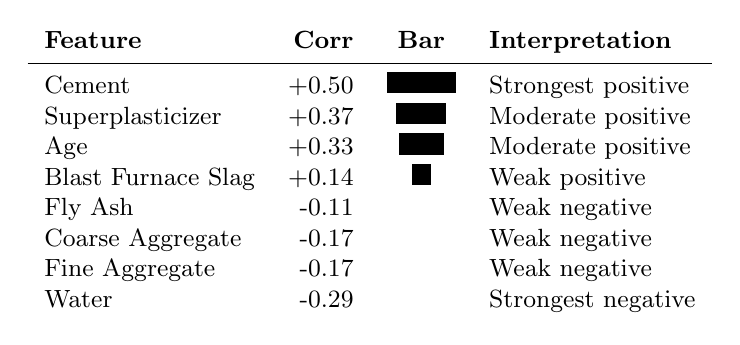
\begin{tikzpicture}[
    node distance=0.5cm,
    every node/.style={font=\small},
    corrbar/.style={rectangle, inner sep=1pt}
  ]
  \node[anchor=south west, inner sep=0] at (0,0) {
    \begin{tabular}{l r c l}
      \textbf{Feature} & \textbf{Corr} & \textbf{Bar} & \textbf{Interpretation} \\
      \midrule
      Cement             &  +0.50 & \rule{25pt}{2ex} & Strongest positive \\
      Superplasticizer   &  +0.37 & \rule{18pt}{2ex} & Moderate positive \\
      Age                &  +0.33 & \rule{16pt}{2ex} & Moderate positive \\
      Blast Furnace Slag &  +0.14 & \rule{7pt}{2ex}  & Weak positive \\
      Fly Ash            &  -0.11 & \rule{-5pt}{2ex} & Weak negative \\
      Coarse Aggregate   &  -0.17 & \rule{-8pt}{2ex} & Weak negative \\
      Fine Aggregate     &  -0.17 & \rule{-8pt}{2ex} & Weak negative \\
      Water              &  -0.29 & \rule{-14pt}{2ex} & Strongest negative \\
    \end{tabular}
  };
\end{tikzpicture}
\end{center}
\begin{center}
\textbf{Figure 4: Correlation between features and strength}
\end{center}

\textbf{Discussion:}
Cement is the strongest predictor, which makes engineering sense: more cement generally means stronger concrete.  Water has a negative correlation, which also makes sense: excess water weakens concrete.  These correlations are consistent with domain knowledge.

However, correlations do not tell us about the \emph{time-dependent} nature of strength.  Age has a moderate positive correlation (+0.33), but this is confounded by the fact that most data is at 28 days.  We need to look at strength \emph{within each mixture} over time, not just across all data.

% -----------------------------------------------------------
\subsection{Experiment 6: Outlier Detection}
\label{sec:experiment-6}

\textbf{Objective:} Identify outliers in strength using the IQR method.

\textbf{OpenCode prompt:}
\begin{lstlisting}[style=term]
Use the IQR method to detect outliers in the target variable.
Report:
- Number of outliers
- Details of outlier observations
- Strength distribution summary (min, max, mean, median, 70th percentile)
\end{lstlisting}

\textbf{Expected results:}
\begin{itemize}[nosep]
  \item 4 outliers detected (strength > 79.77 MPa)
  \item Strength range: 2.33 -- 82.60 MPa
  \item Mean: 35.82 MPa, Median: 34.45 MPa
  \item 70th percentile: 43.29 MPa (70\% of data below this)
\end{itemize}

\textbf{Discussion:}
The strength distribution is right-skewed: the mean (35.82) is higher than the median (34.45), and the 70th percentile is only 43.29 MPa.  This means most concrete in the dataset has moderate strength (10--50 MPa), with a few high-strength examples.  Outliers may represent high-performance concrete mixes, which could be an interesting subpopulation to explore further.

% -----------------------------------------------------------
\subsection{Experiment 7: Data Imbalance Summary}
\label{sec:experiment-7}

\textbf{Objective:} Group observations into time bins and understand the temporal distribution.

\textbf{OpenCode prompt:}
\begin{lstlisting}[style=term]
Group observations into time bins:
- Early (1--7 days)
- Standard (8--28 days)
- Medium (29--90 days)
- Long (91--180 days)
- Very Long (181+ days)
Report the count and percentage in each bin.
\end{lstlisting}

\textbf{Expected results:}
\begin{center}
\begin{tabular}{l r r}
\toprule
\textbf{Bin} & \textbf{Count} & \textbf{\%} \\
\midrule
Early (1--7 days)     & 262 & 25.4\% \\
Standard (8--28 days) & 487 & 47.3\% \\
Medium (29--90 days)  & 145 & 14.1\% \\
Long (91--180 days)   & 103 & 10.0\% \\
Very Long (181+ days) &  33 &  3.2\% \\
\bottomrule
\end{tabular}
\end{center}

\textbf{Discussion:}
Nearly half the data (47.3\%) is in the 8--28 day range.  Only 3.2\% is for very long curing times (181+ days).  This imbalance means:
\begin{itemize}[nosep]
  \item Models will be well-calibrated for short-to-medium curing times
  \item Predictions for long-term strength will have high uncertainty
  \item Standard evaluation metrics (e.g., MSE on the full dataset) will be dominated by performance at 28 days
\end{itemize}

% ===========================================================
\section{What We Learned}
\label{sec:learnings}

Through these seven experiments, we have discovered four key facts about the concrete dataset:

\begin{enumerate}[nosep]
  \item \textbf{Supervised setting exists but is challenging.}  The data provides features and a target, but the relationship is highly nonlinear and time-dependent.
  
  \item \textbf{Sparsity is extreme.}  96.3\% of (mixture, age) combinations appear only once.  Most mixtures have only 1--3 age measurements.
  
  \item \textbf{Age imbalance is severe.}  47.3\% of data is at 28 days; only 3.2\% is for long-term curing (181+ days).
  
  \item \textbf{Physics matters.}  Strength evolves with age according to curing kinetics, not as a simple feature--target mapping.  Treating Age as just another feature ignores this physics.
\end{enumerate}

These findings have important implications for modeling:

\begin{def-box}
\textbf{Naive approach (treat Age as feature):}  Train a standard regression model with all 8 features (7 components + Age).  This will work reasonably well for 28-day predictions but will fail for other ages because the model has no mechanism to capture the time-dependent curing process.
\end{def-box}

\begin{def-box}
\textbf{Better approach (physics-informed):}  Use domain knowledge to inform the model.  For example, use log(Age) instead of Age, or fit separate models for different subpopulations (e.g., mixtures with vs. without slag).  This requires more engineering effort but will generalize better.
\end{def-box}

\begin{def-box}
\textbf{Best approach (hierarchical / mixed-effects):}  Treat each mixture as a random effect with a shared curing curve.  This leverages the growth curve data (76\% of rows) while accounting for the sparsity per mixture.  This is the most statistically sound approach but requires careful implementation.
\end{def-box}

In future tutorials, we will explore these approaches in more detail.  For now, the key takeaway is: \textbf{understanding the data is the first and most important step in any ML project.}  Without this understanding, you risk building models that are statistically convenient but scientifically meaningless.

% ===========================================================
\section{Creating Your SKILL}
\label{sec:skill}

Now that you have explored the data, it is time to create a \textbf{SKILL} artifact.  A SKILL is a reusable piece of knowledge that captures what you have learned and can be applied to future similar problems.

\begin{def-box}
\textbf{What is a SKILL?}  A SKILL is a Markdown file that documents:
\begin{itemize}[nosep]
  \item \textbf{Purpose:} When to use this skill (what kind of data/problems it applies to)
  \item \textbf{Key observations:} The main challenges or patterns you discovered
  \item \textbf{Exploration checklist:} Step-by-step prompts you can use to explore similar data
  \item \textbf{Discussion questions:} Questions to help you think critically about the results
  \item \textbf{What to try next:} Suggestions for modeling approaches
\end{itemize}
\end{def-box}

\textbf{Your task:} Create a Markdown file called \texttt{concrete-sparsity-skill.md} in the tutorial directory.  Use the following structure:

\begin{lstlisting}[style=term]
# Concrete Sparsity Exploration Skill

## Purpose
When to use this skill (sparse longitudinal data with physical time dimension)

## Key Observations
The 4 challenges: supervised setting exists, time != feature, sparse per mixture, age imbalance

## Exploration Checklist
Step-by-step OpenCode prompts for similar datasets

## Discussion Questions
Prompts for class discussion

## What to Try Next
Suggest modeling approaches without implementing

## References
Link to dataset readme and original papers
\end{lstlisting}

\textbf{Guidelines:}
\begin{itemize}[nosep]
  \item Use the findings from your exploration (sparsity ratio, age distribution, etc.)
  \item Make the exploration checklist \emph{general} --- it should apply to any sparse longitudinal dataset, not just concrete
  \item Include the OpenCode prompts you used, but generalize them for other data
  \item Do \emph{not} include code implementation (this is a discussion-only tutorial)
\end{itemize}

\begin{alert-box}
\textbf{This SKILL is your empirical knowledge.}  It captures what you learned through trial-and-error exploration.  When you encounter a similar dataset in the future, you can use this SKILL to guide your exploration efficiently.  This is the transition from one-off learning to \emph{reusable expertise}.
\end{alert-box}

\begin{ex-box}
\textbf{Example SKILL prompt for OpenCode:}
\begin{lstlisting}[style=term]
Create a Markdown file called concrete-sparsity-skill.md with the following structure:
- Purpose: When to use this skill
- Key Observations: The 4 challenges
- Exploration Checklist: Step-by-step OpenCode prompts
- Discussion Questions: Prompts for class discussion
- What to Try Next: Suggest modeling approaches
- References: Links to dataset and papers
\end{lstlisting}
\end{ex-box}

% ===========================================================
\section{Looking Ahead}
\label{sec:outlook}

\begin{def-box}
Through this tutorial you have learned to use OpenCode for \emph{systematic data exploration}.  You discovered that real-world data is often sparse, imbalanced, and challenging to model.  You created a SKILL artifact that captures this empirical knowledge.

\medskip
\noindent\textbf{What comes next?}
\begin{enumerate}[nosep]
  \item \textbf{Modeling sparse longitudinal data.}  In future tutorials, we will explore approaches like log-transforming Age, using hierarchical models, and incorporating domain knowledge.
  \item \textbf{Evaluation strategies.}  How do we evaluate models when data is sparse and imbalanced?  Standard metrics (MSE, $R^2$) may be misleading.
  \item \textbf{Tool orchestration.}  As you become more comfortable with OpenCode, you will learn to chain multiple tools (view, bash, edit) into coherent pipelines.
  \item \textbf{Human--AI orchestration.}  The most important skill is knowing \emph{when} to let the agent act and \emph{when} to take the wheel yourself.  You will develop judgment for delegating, reviewing, and overriding agent decisions.
\end{enumerate}

\medskip
\noindent The SKILL you create in this tutorial is the first step toward building a \emph{personal knowledge base} of empirical insights.  Over time, these skills will accumulate and become your most valuable asset as a practitioner of AI in engineering.
\end{def-box}

% ===========================================================
% References
% ===========================================================

\begin{thebibliography}{9}

\bibitem{yeh1998}
I-Cheng Yeh, ``Modeling of strength of high performance concrete using artificial neural networks,'' \emph{Cement and Concrete Research}, Vol.~28, No.~12, pp.~1797--1808 (1998).

\bibitem{opencode2025}
opencode-ai, ``OpenCode: A powerful AI coding agent. Built for the terminal,'' \emph{GitHub}, 2025. Available: \url{https://github.com/opencode-ai/opencode}

\bibitem{opencode_readme2025}
opencode-ai, ``OpenCode README --- Configuration, Usage, and Keyboard Shortcuts,'' \emph{GitHub}, 2025. Available: \url{https://github.com/opencode-ai/opencode/blob/main/README.md}

\bibitem{opencode_install2026}
OpenCode, ``Install script,'' \emph{opencode.ai}, 2026. Available: \url{https://opencode.ai/install}

\bibitem{microsoft_wsl2026}
Microsoft, ``Windows Subsystem for Linux Documentation,'' \emph{Microsoft Learn}, 2026. Available: \url{https://learn.microsoft.com/en-us/windows/wsl/}

\end{thebibliography}

\end{document}
